% !TEX root = ../tjumain.tex

\chapter{实验结果及分析}

\section*{实验测试环境}

通过 VirtualBox 虚拟机进行测试,脚本默认丢包率 6\%,延迟 6ms。系统环境如图\ref{fig:ubuntu} 所示。测试方法是使用脚本和修改后的测试脚本进行运行,分析输出的log进行debug。

\section{连接建立的功能测试与结果分析}

连接建立的Log文件如图\ref{fig:established_log}所示:

\begin{figure}[!htbp]
    \centering
    \subfigure[server 端]{\includegraphics*[width=0.45\textwidth]{e_server1.png}\label{fig:e_server}}
    \subfigure[client 端]{\includegraphics*[width=0.45\textwidth]{e_client1.png}\label{fig:e_client}}
    \caption{连接创建 Log }\label{fig:established_log}
  \end{figure}

可以看到,Client 端首先创建了第一个 SYN 报文并进行发送,然后由于初次设置的 Timer 并不合理,立马出现了 timeout,进行重传,在接收到 SYN | ACK 后确认建立全连接,并发送 ACK 同时删除一个 timer 。 Server 端接收到 SYN 报文后进行 SYN | ACK 的返回,最后接受到 ACK 后确定一个 Full Connection 的建立。

\section{可靠传输的功能测与结果分析}

\subsection{RTO动态调整}
如图\ref{fig:RTTFIG} 是在 100Mbps 20ms 延迟的情况下观测到的数据,可见,我们的 TimeoutInterval 的确是随事件变化、随EstimatedRTT变化的。

\begin{figure}[!htbp]
    \centering
    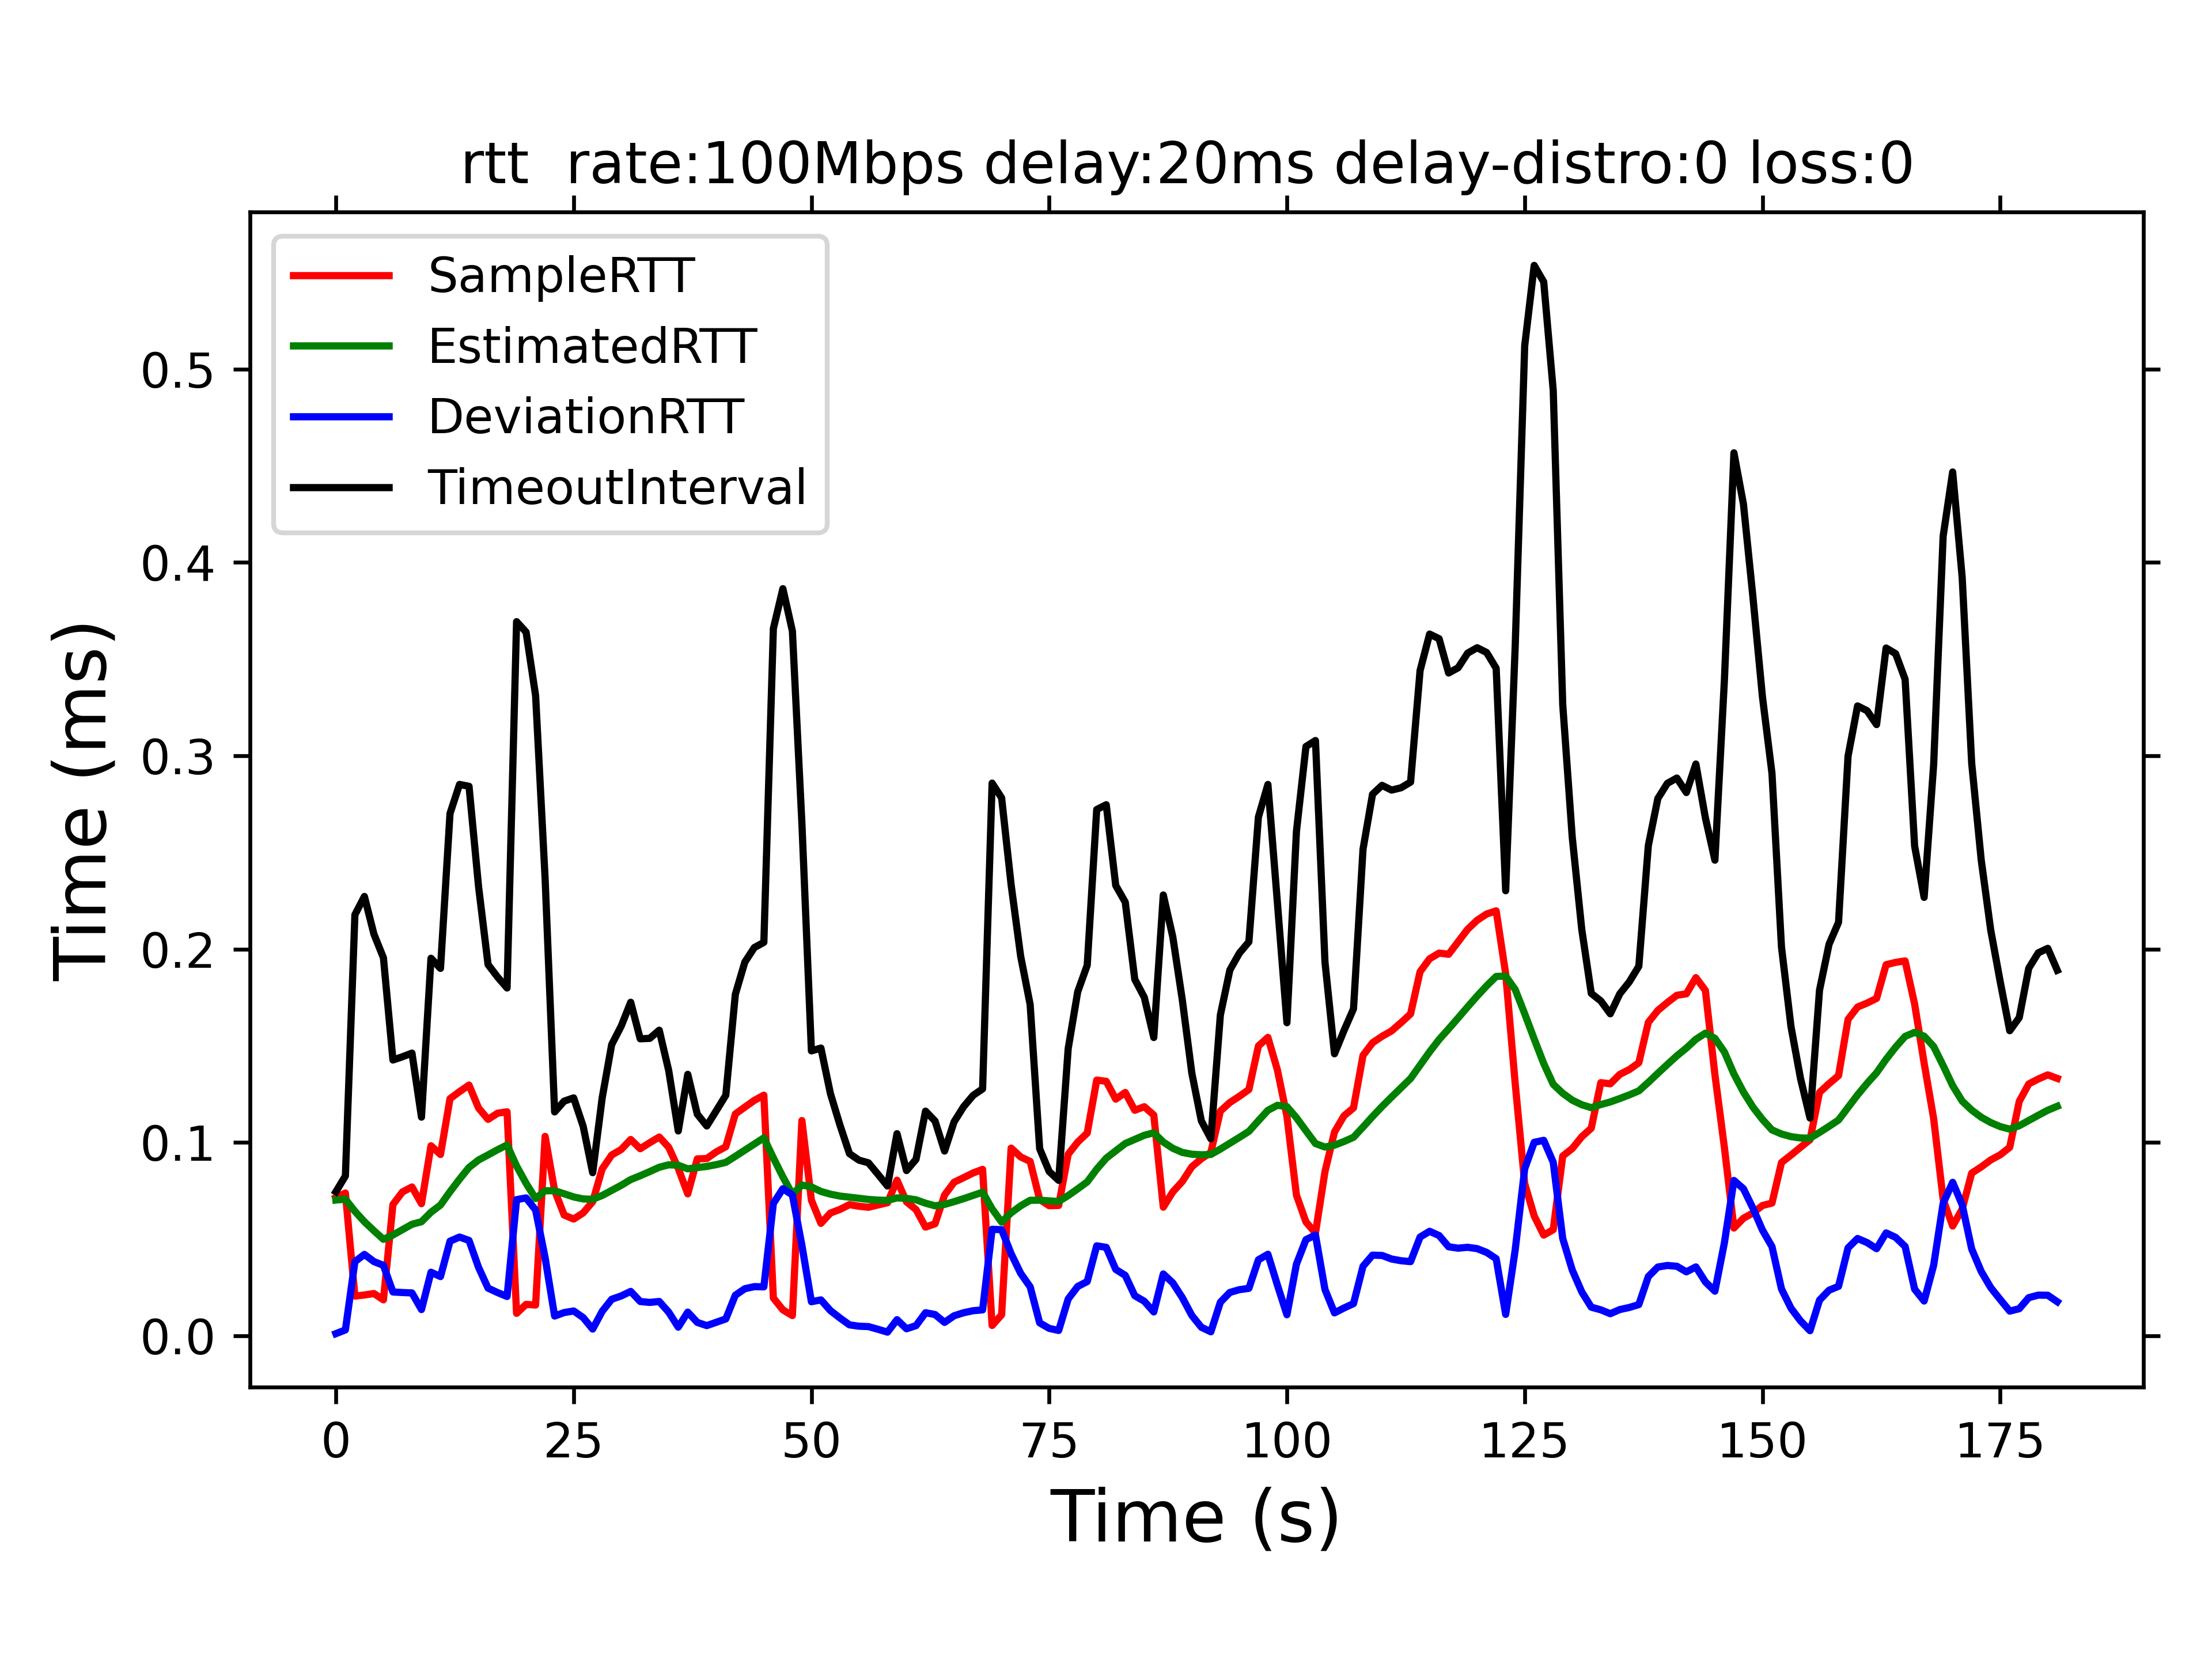
\includegraphics[width=5.5in]{RTT_FIG.png}
    \caption{RTT动态调整 图}\label{fig:RTTFIG}
\end{figure}

如图\ref{fig:RTTLOG}是 RTO 根据获得的 EstimatedRTT 进行的调整
\begin{figure}[!htbp]
    \centering
    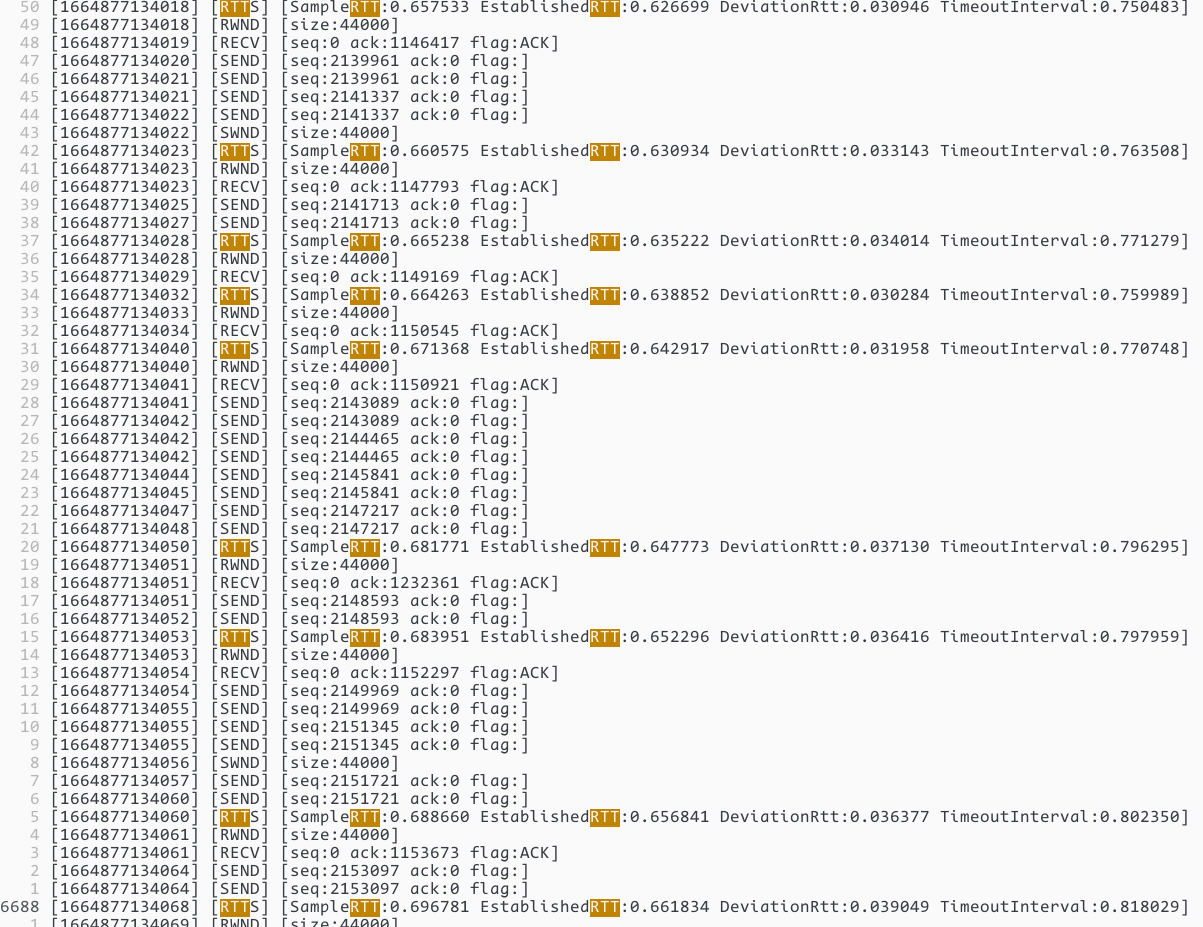
\includegraphics[width=5.5in]{RTT_LOG.png}
    \caption{RTT动态调整 Log}\label{fig:RTTLOG}
\end{figure}

\subsection{可靠数据传输}

我们通过 Client 端的 Trace (如图\ref{fig:recvLog})可以看到接受到连续 ACK 表明接收到了正确的信息。更多测试,在后续的性能中进行展示。

\begin{figure}[!htbp]
    \centering
    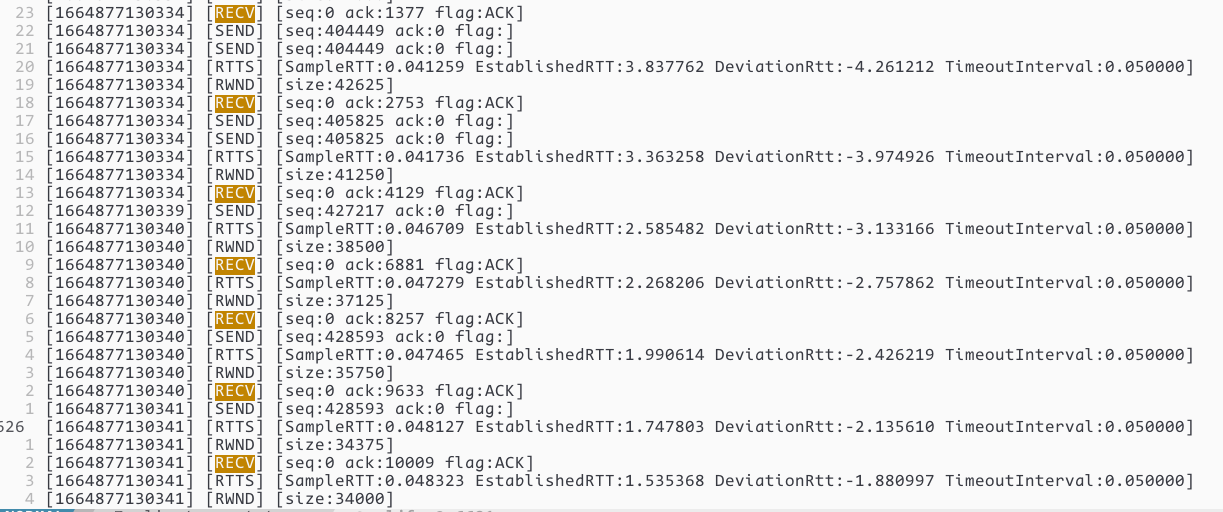
\includegraphics[width=5.5in]{RECV_LOG.png}
    \caption{接收 Seq 跟随变化图}\label{fig:recvLog}
\end{figure}

\section{流量控制的功能测试与结果分析}


为最大限度地选出优秀的结果,我们将家庭NAS服务器系统装上了 Arch Linux 并安装 vagrant 等进行大量脚本测试,跑出了 1728 个结果(如图\ref{fig:results_all}),精选后,我们选出一个较为优秀的结果精选展示。

\begin{figure}[!htbp]
    \centering
    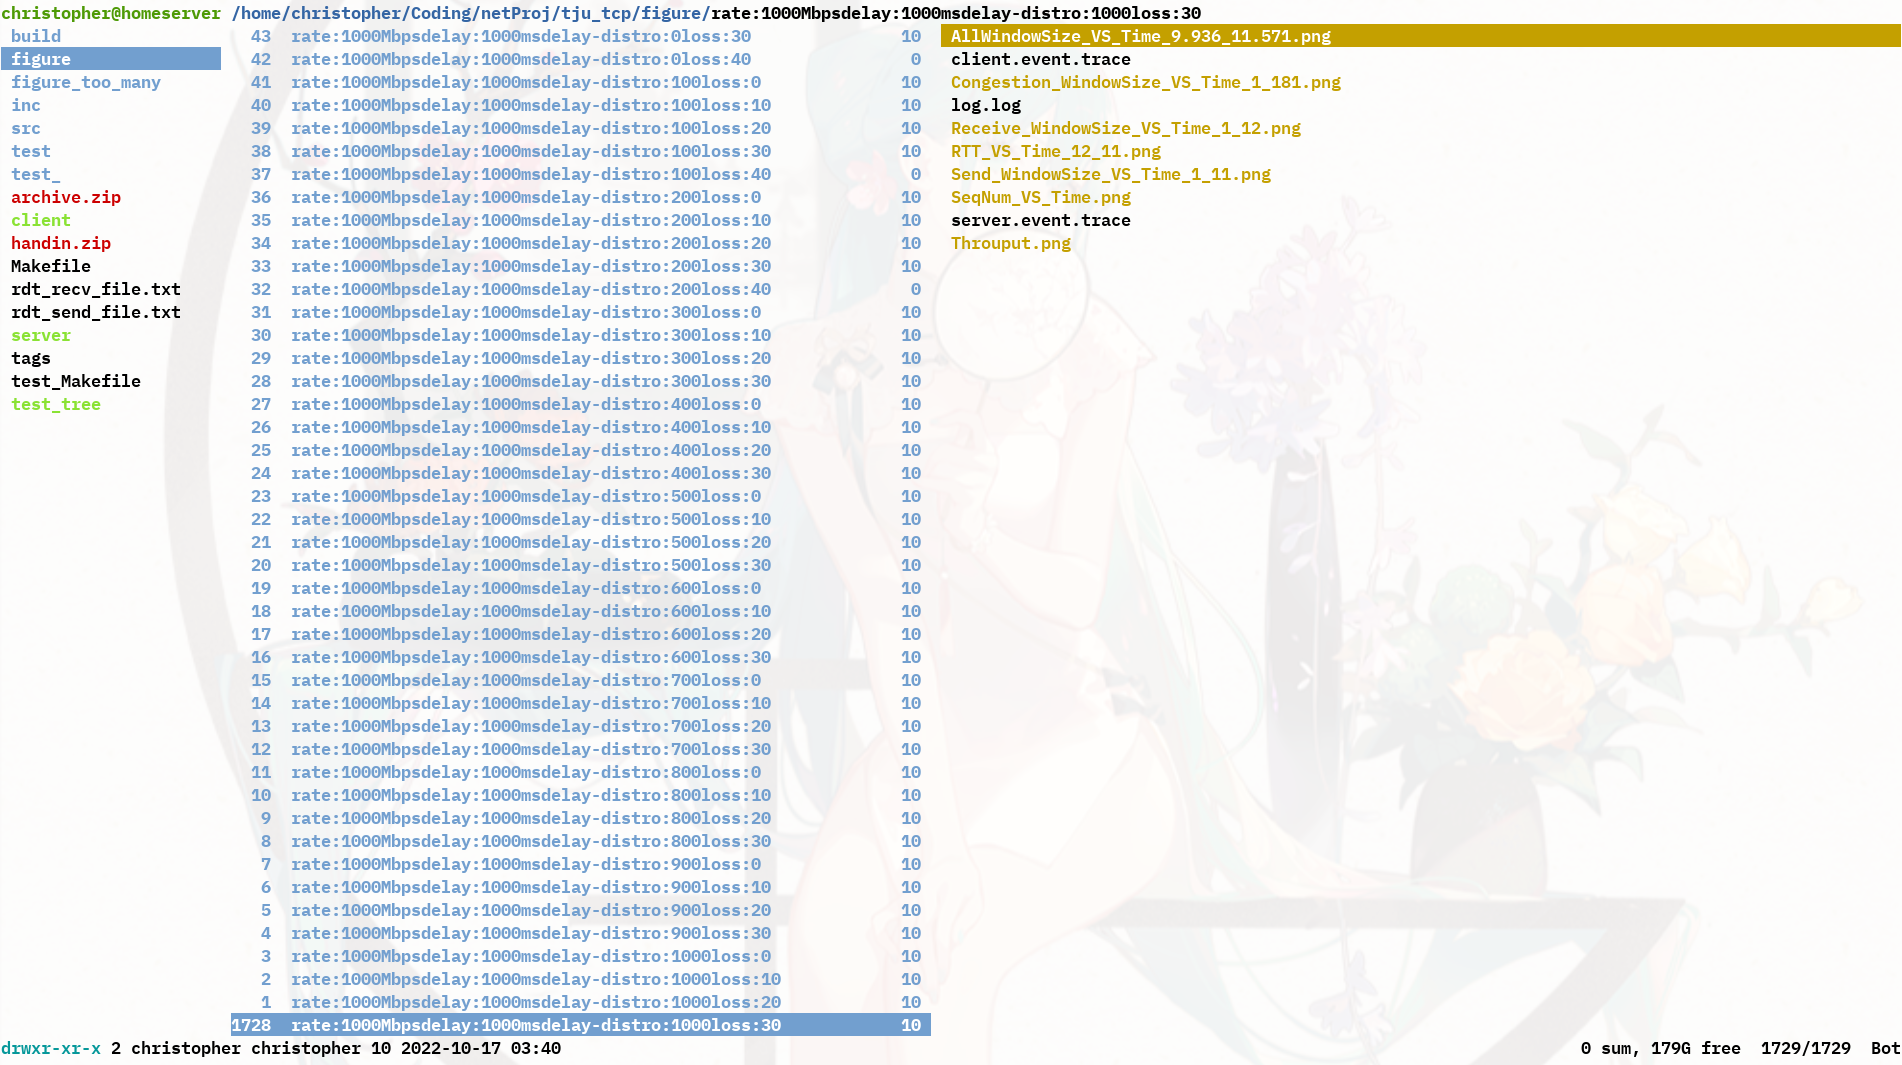
\includegraphics[width=5.5in]{homeserver.png}
    \caption{家庭NAS系统结果}\label{fig:results_all}
\end{figure}


我们选出在100Mbps 20ms 延迟环境下的测试结果\ref{fig:all_window}。显示我们的流量控制效果是合理的,能够将窗口的变化实时体现在 swnd 中。
\begin{figure}[!htbp]
    \centering
    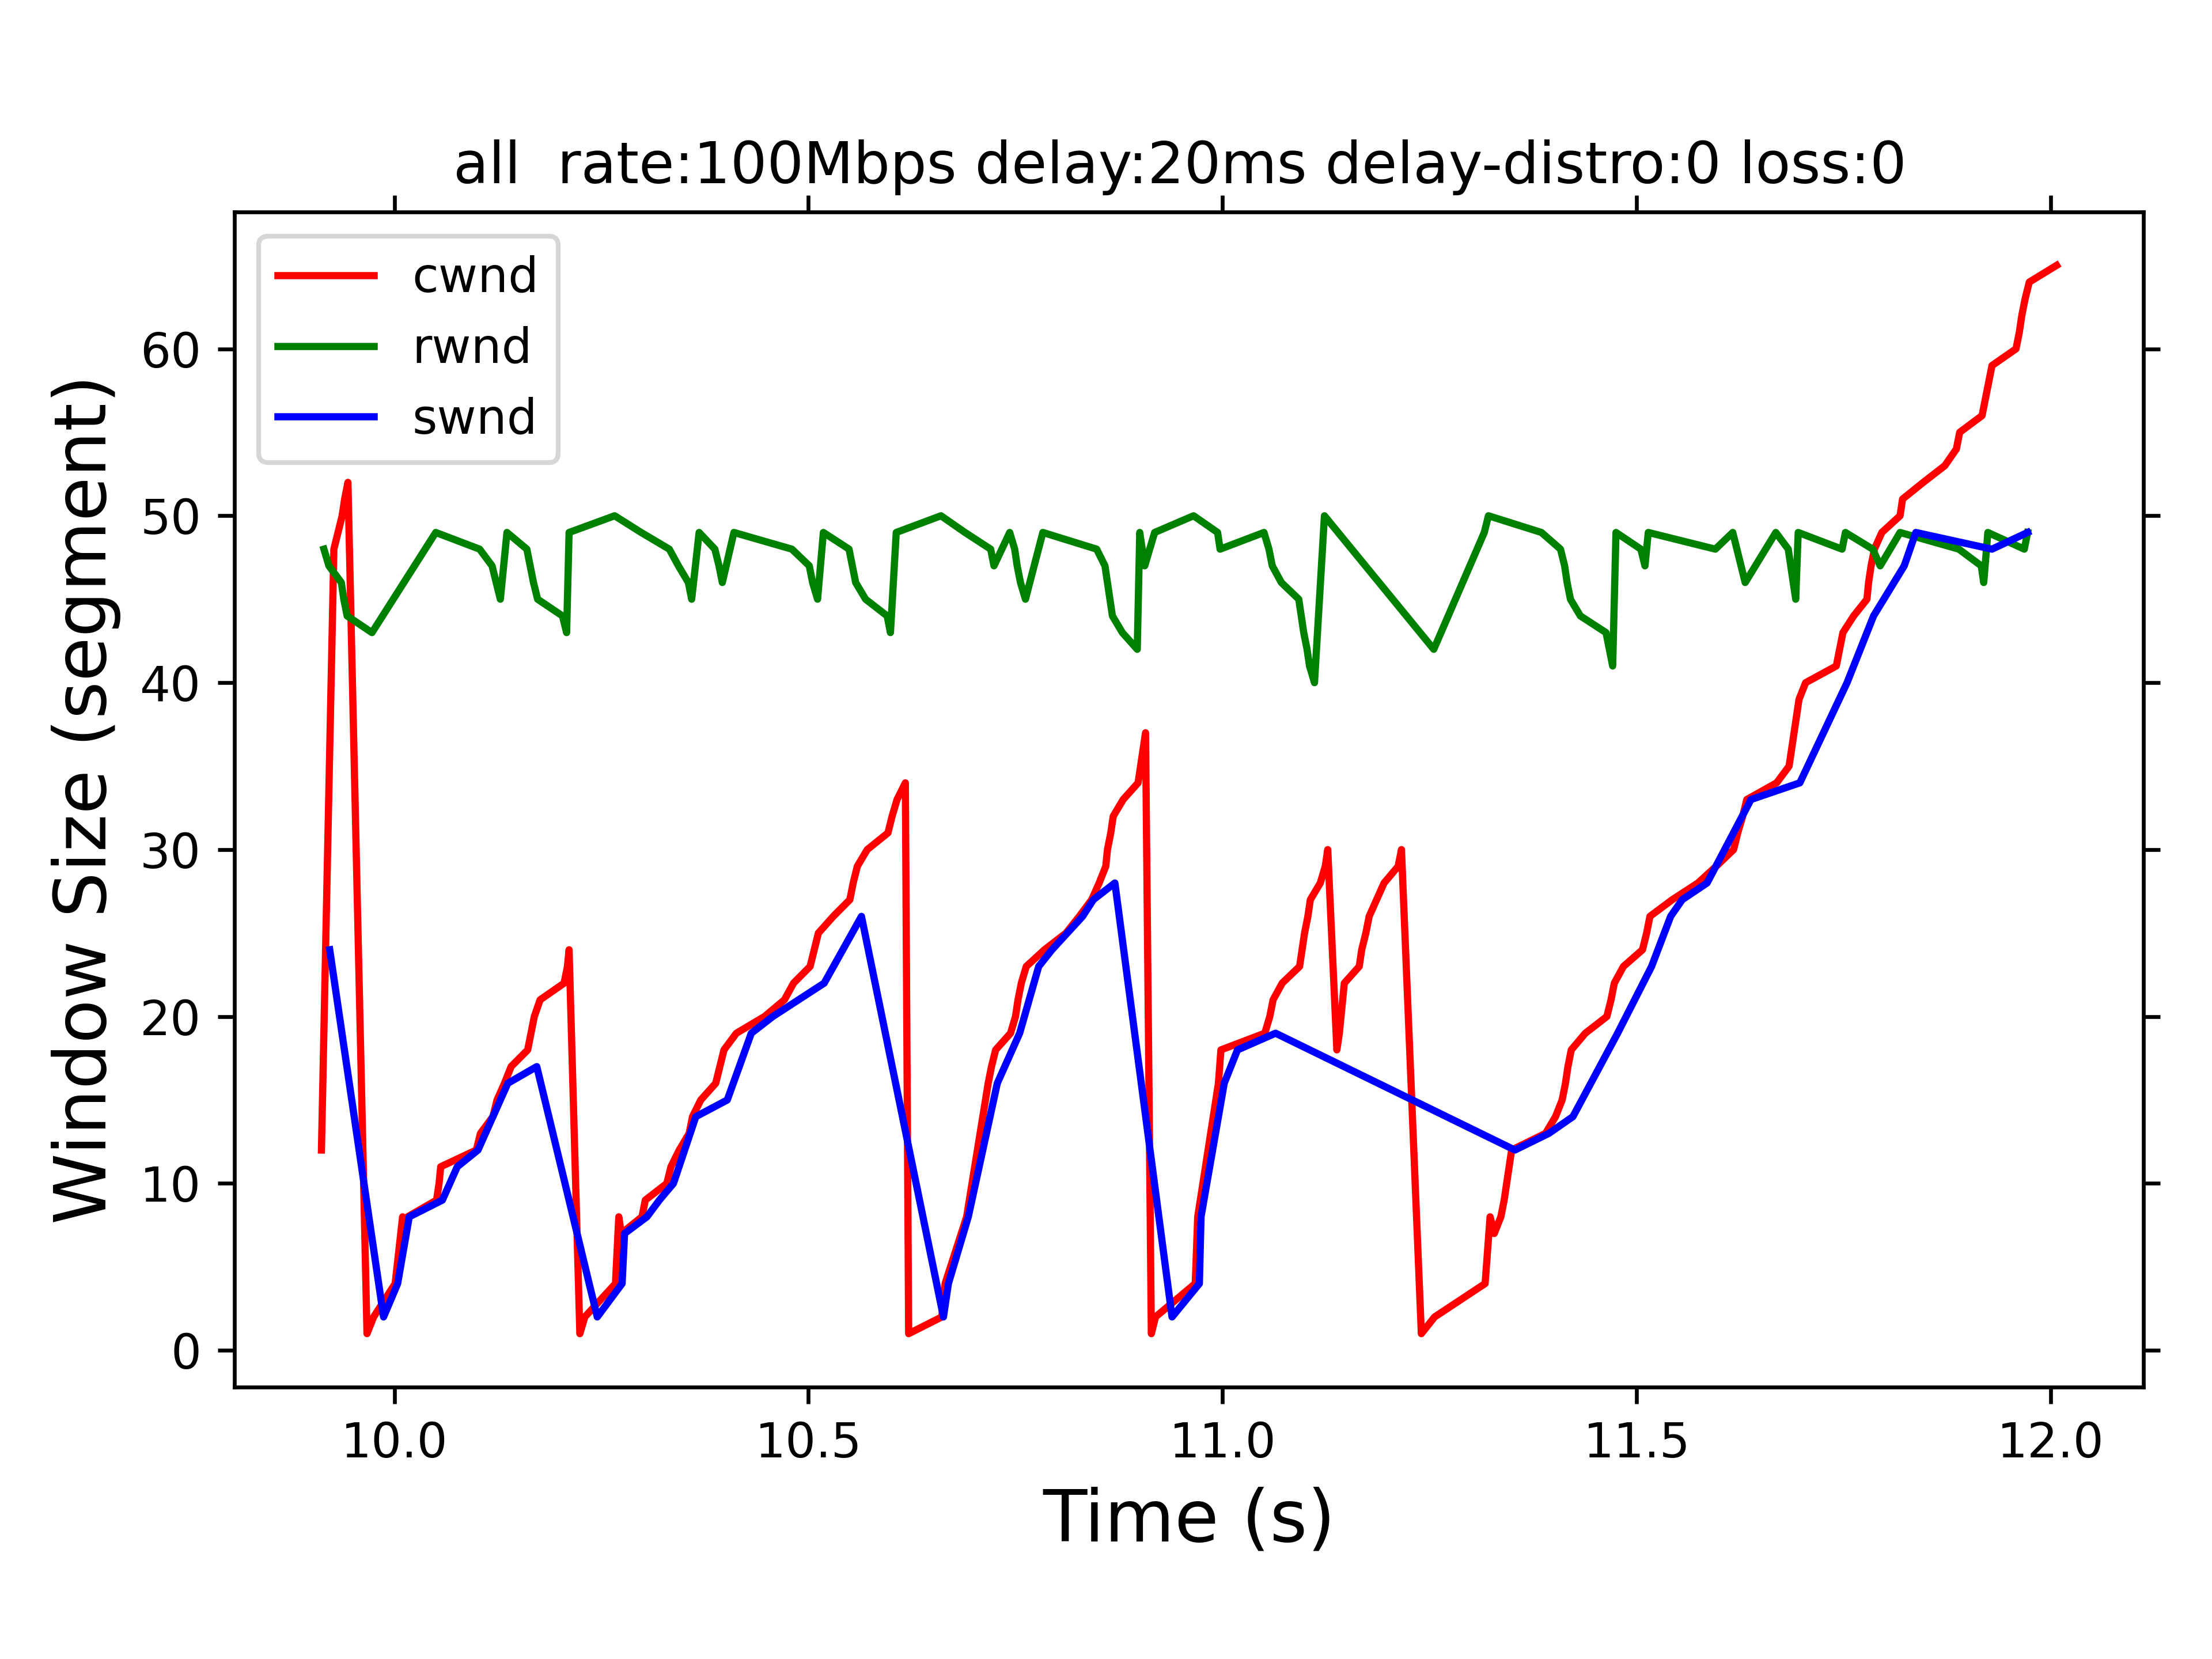
\includegraphics[width=5.5in]{all_window.png}
    \caption{流量控制}\label{fig:all_window}
\end{figure}

\section{连接关闭的功能测试与结果分析}
我们顺利在 Auto Lab 上提交了正确答案,确实没太多特性需要测试,在此附上一个 AutoLab上的截图证明(如图\ref{fig:close_test})。

\begin{figure}[!htbp]
    \centering
    
\includegraphics[width=4in]{close_test.png}
    \caption{连接关闭证明}\label{fig:close_test}
\end{figure}

\section{拥塞控制的功能测试与结果分析}
经过脚本测试,我们选出了在环境100Mbps 20ms延迟的数据进行展示,可以看到,我们的cwnd实现能够在正确地情况出现时给予正确的处理:即1. 刚开始时采取慢启动。2. 达到 sshresh 时采取拥塞避免。 3. 在发生超时的同时将窗口大小降低并进行慢启动。4. 出现三次 ack 时降低一般的窗口。整个图形呈现锯齿状

\begin{figure}[!htbp]
    \centering
    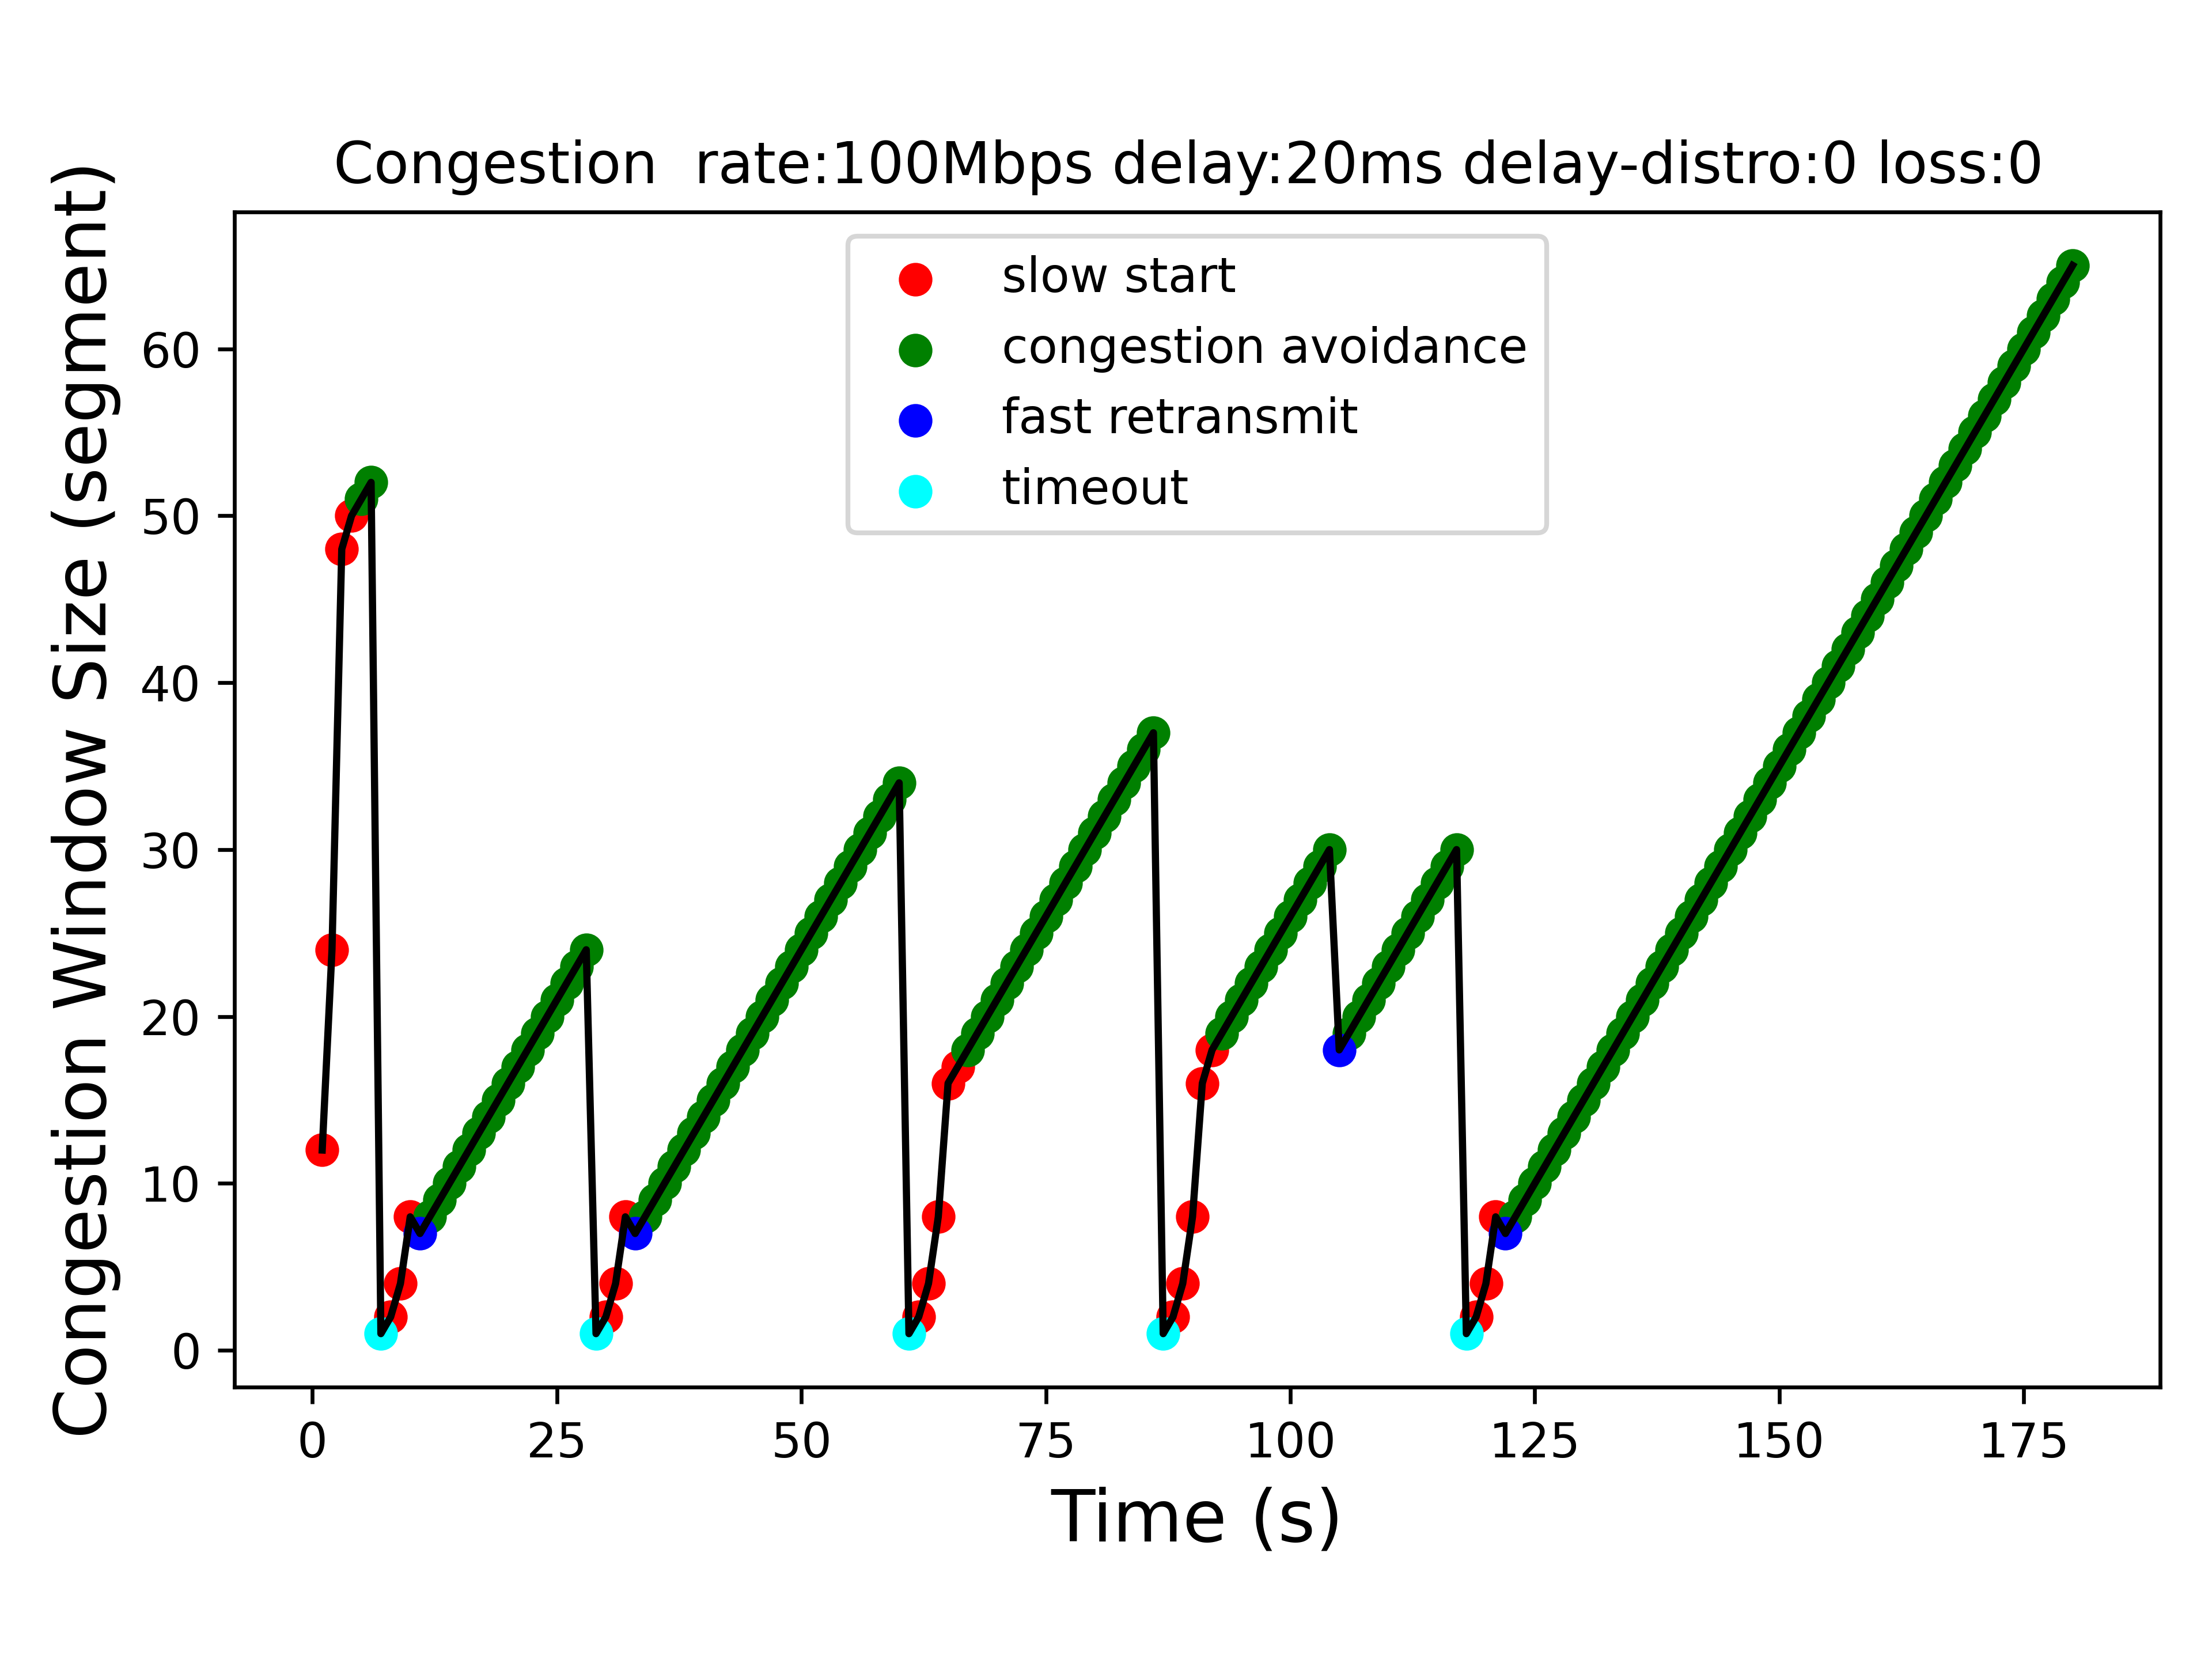
\includegraphics[width=5.5in]{conngestion.png}
    \caption{Congestion窗口变化图}\label{fig:congestion}
\end{figure}

\section{TCP协议性能测试与结果分析}

我们分别对吞吐率-窗口大小和吞吐率-丢包率两种情况做了测试(如图\ref{fig:throughtput-loss}和\ref{fig:throughtput-wds}所示)。

\begin{figure}[!htbp]
    \centering
    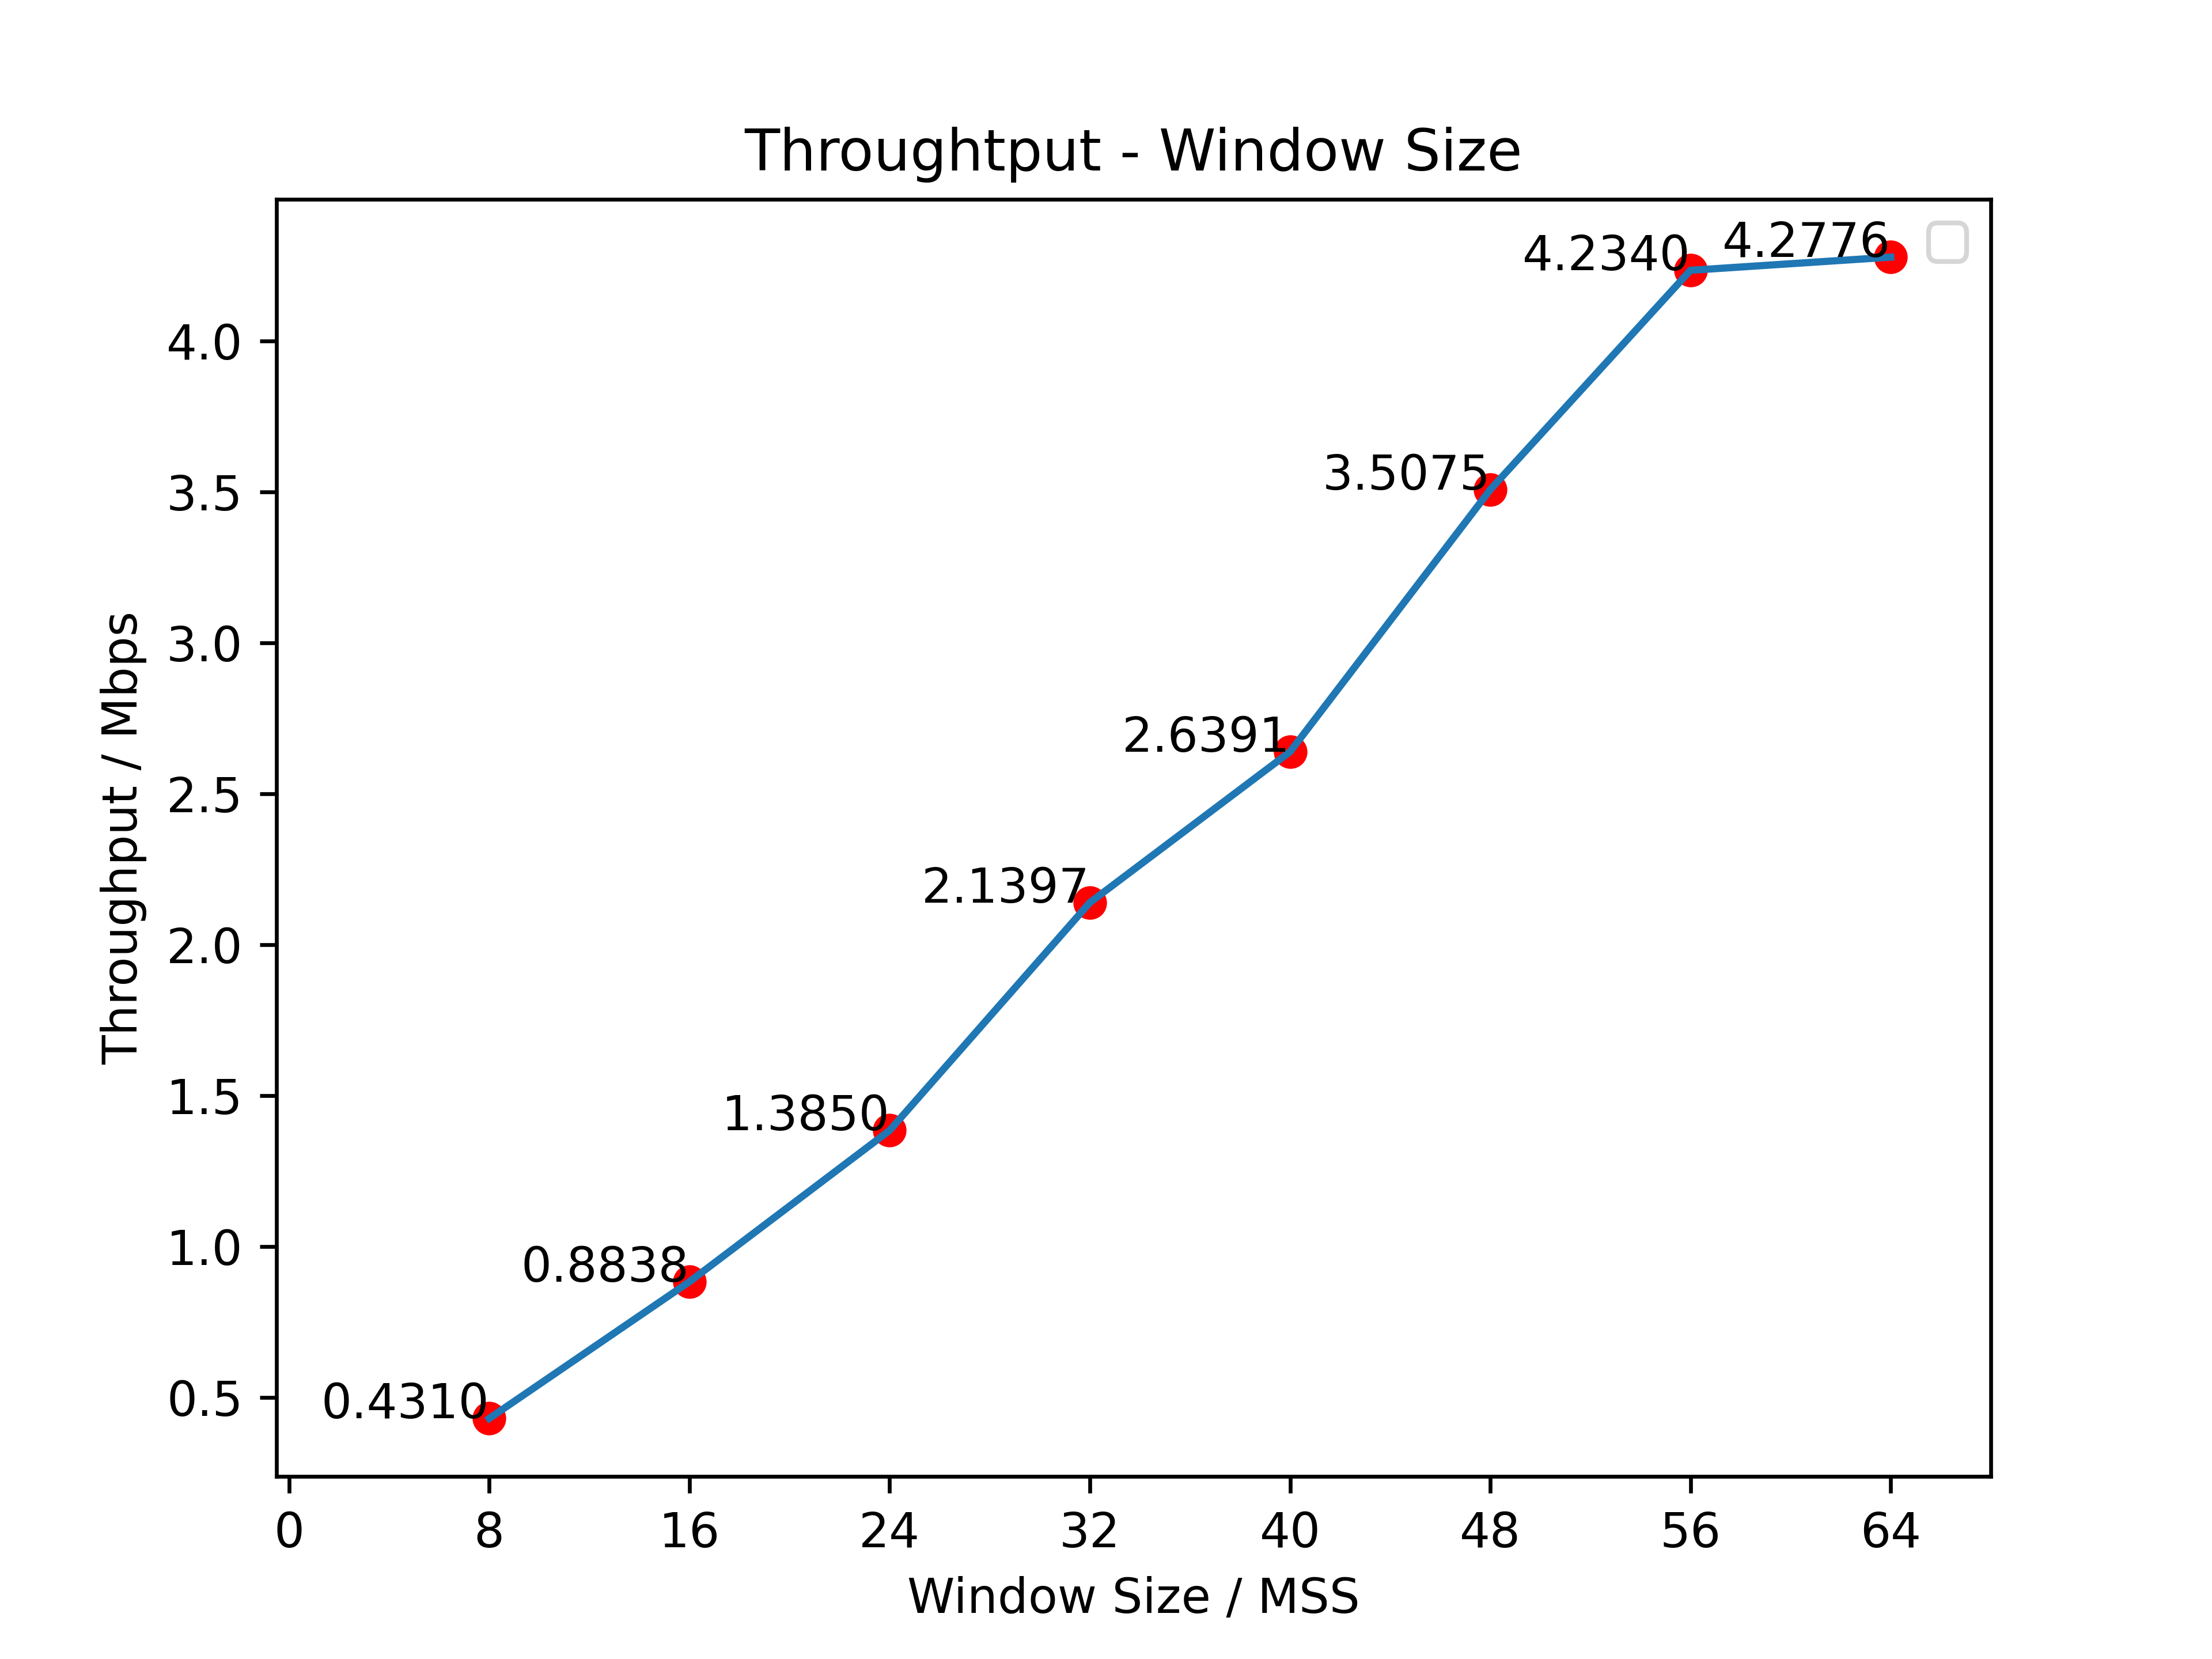
\includegraphics[width=5.5in]{wds.png}
    \caption{吞吐率-窗口大小}\label{fig:throughtput-wds}
\end{figure}


\begin{figure}[!htbp]
    \centering
    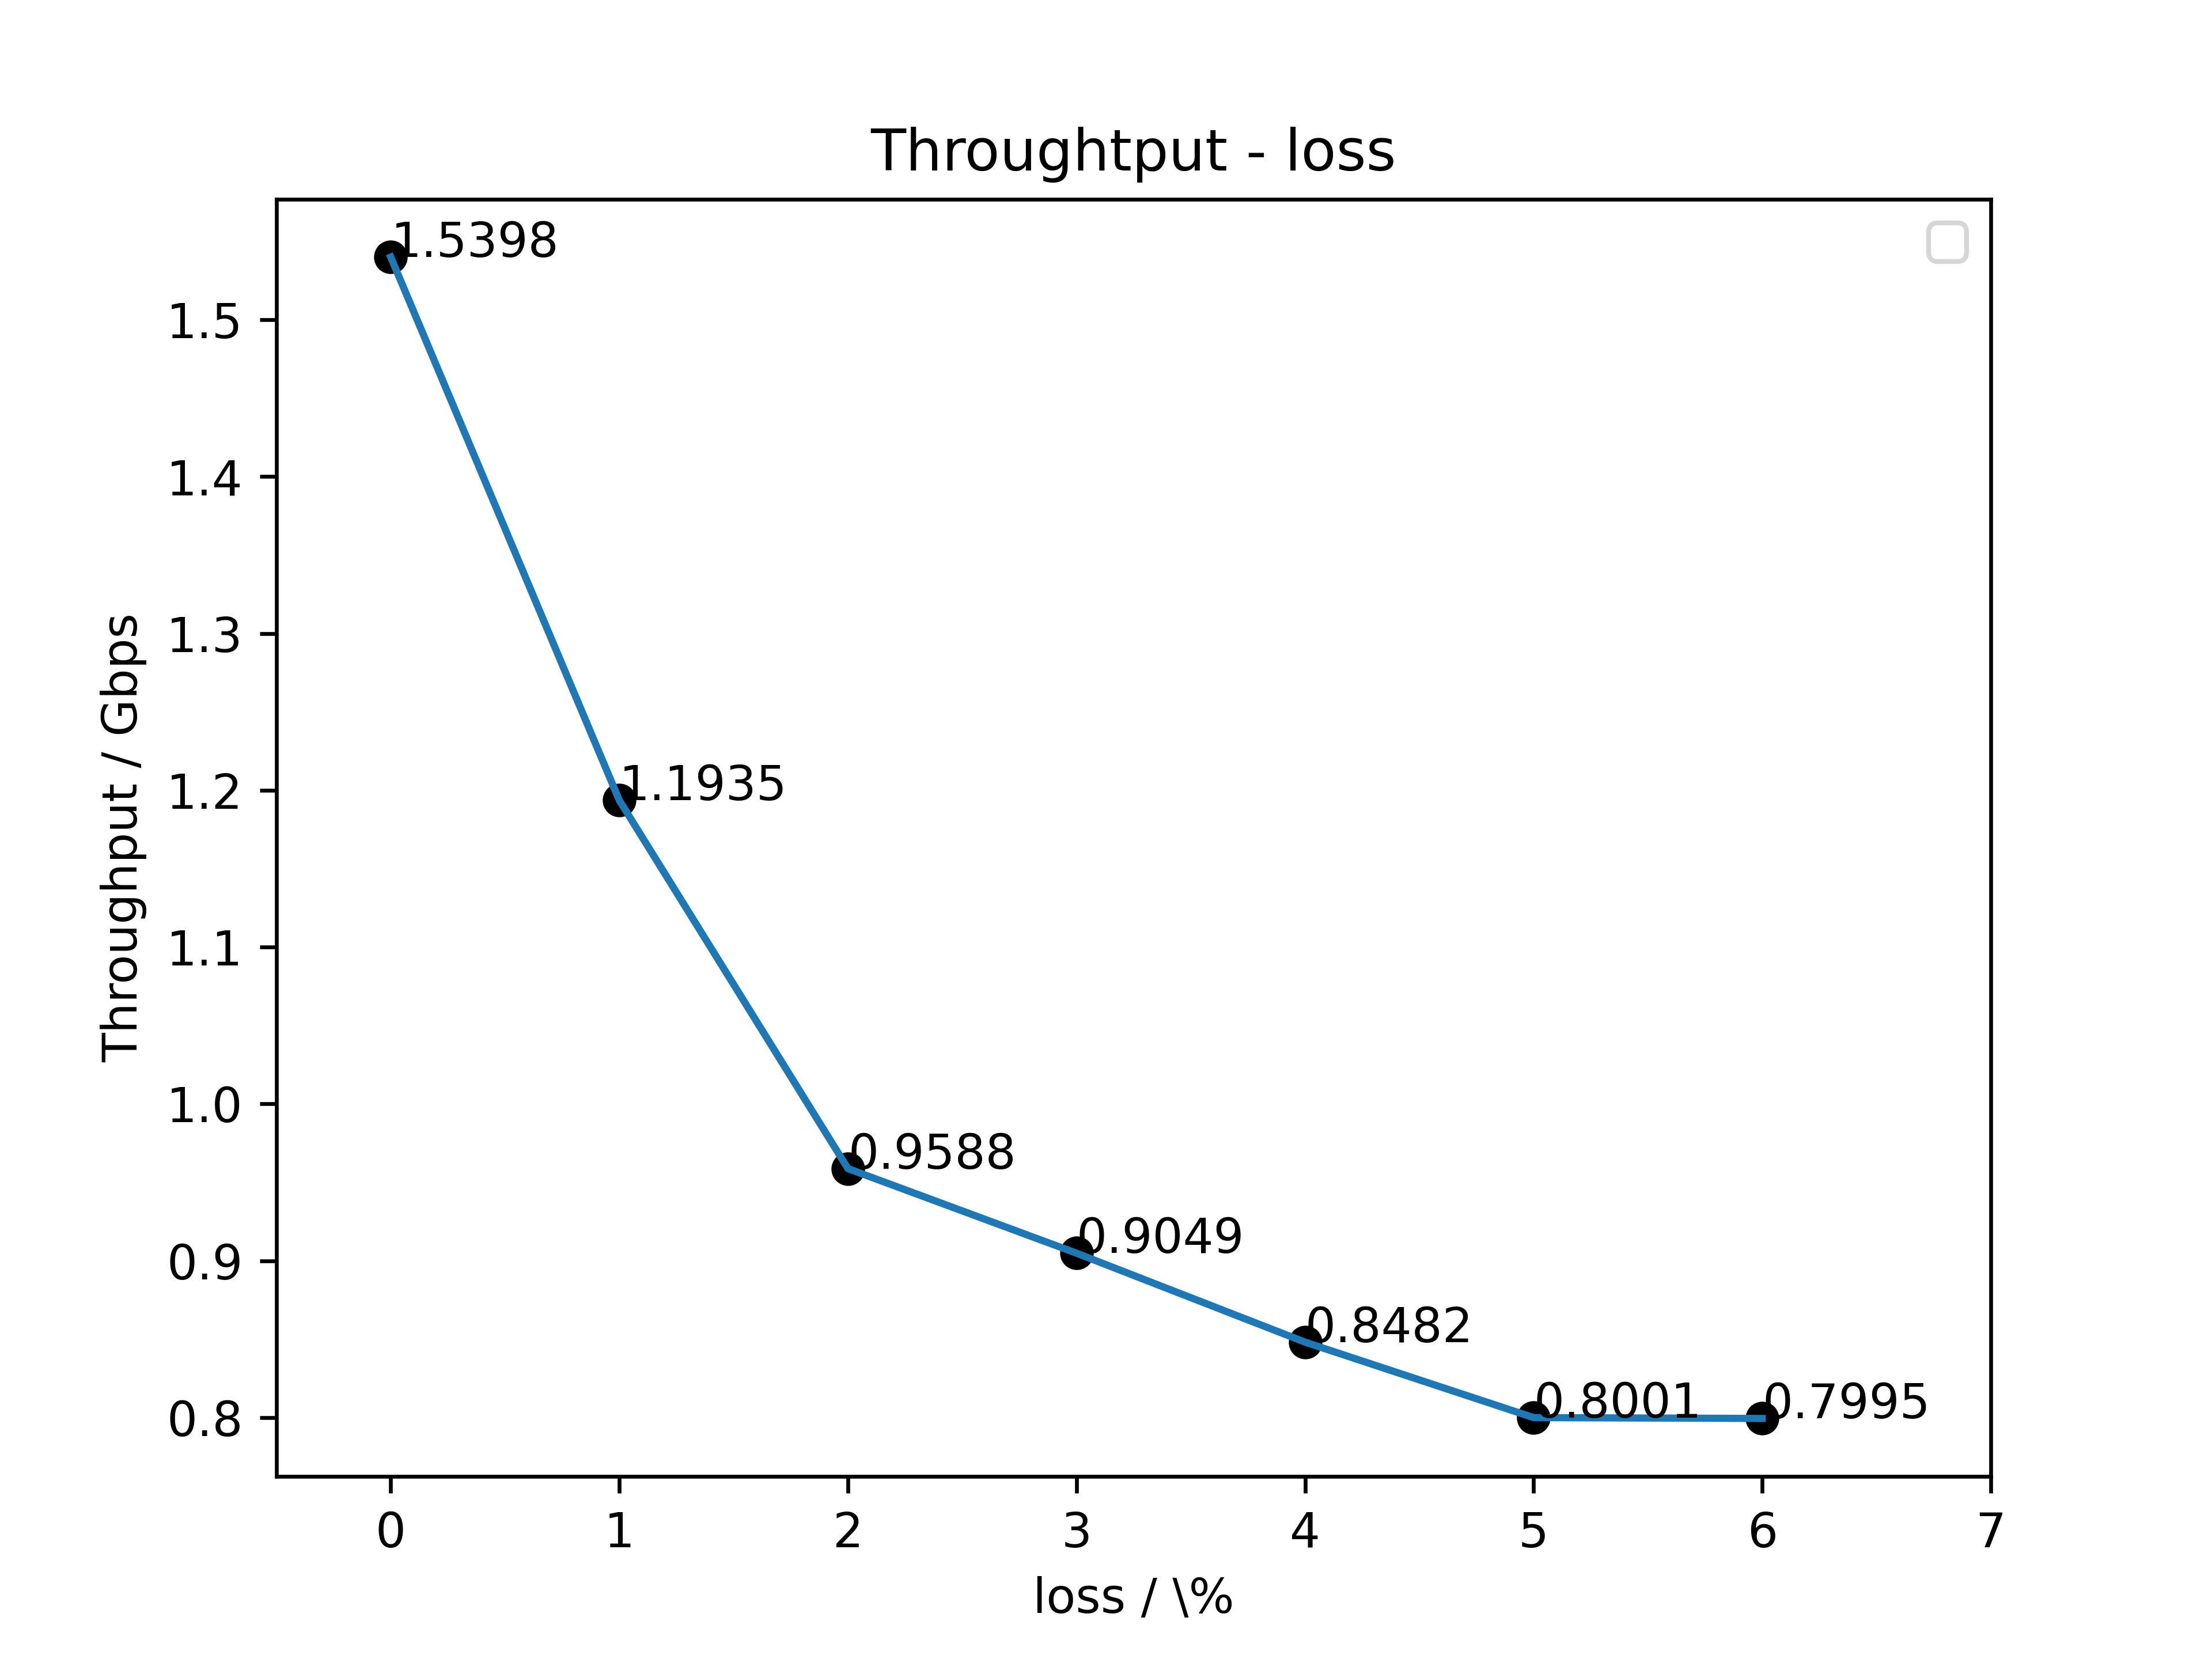
\includegraphics[width=5.5in]{loss.png}
    \caption{吞吐率-丢包率}\label{fig:throughtput-loss}
\end{figure}

\paragraph*{窗口大小} 可见,随着窗口大小的增加,吞吐率有明显地增大。但在较大的两个数据:56和64之间的吞吐率差距较小。这可能是因为我们仍然设置了对发送缓冲区的大小做了限制:即发送端在发送缓冲区满的时候需要停下来等待。且每次都需要对环境进行加锁、解锁,这些流程也会使得整体速率是有上限的。也就是说我们的表现是正确的。

\paragraph*{丢包率} 可见,吞吐率随着丢包率的提高而下降,我们选取的窗口大小为32,符合图\ref{fig:throughtput-wds} 的数据。同时,在产生1\%丢包率时,其吞吐率相较没有丢包率时有明显的下降。这表明在 TCP 现在的标准下,产生丢包等误判会严重降低吞吐率,我们或许有更好的设计思路能够提升这一情况下的吞吐率。





